\documentclass{article}
\usepackage{template}
\usepackage{array}
\usepackage{pgfgantt}
\usepackage{graphicx}
\usepackage{authblk}

\newcolumntype{F}[1]{%
    >{\raggedright\arraybackslash\hspace{0pt}}p{#1}}%
\newcolumntype{T}[1]{%
    >{\centering\arraybackslash\hspace{0pt}}p{#1}}%
\usetikzlibrary{positioning}
\renewcommand{\qedsymbol}{\ensuremath{\blacksquare}}
\tikzset{set/.style={draw,circle,inner sep=0pt,align=center}}
\title{\LARGE Mathematical Kaleidoscope III: \\ \large Auxillary Variable Methods}
\author[1]{Anders Malthe Westerkam}
\author[2]{Malte Bødker}
\author[3]{Toke Christian Zinn}
\affil[1]{amw@es.aau.dk}
\affil[2]{maltebn@math.aau.dk}
\affil[3]{tokecz@math.aau.dk}
\begin{document}
\maketitle
\section*{Introduction}
Suppose that for a given random variable $X$, we are interested in computing a certain functional or statistic. For example, we may be interested in computing $\mathbb{E}[f(X)]$ for some appropriate function $f$, for which the expected value is well-defined. Of course, if we can derive the law of $f(X)$ and subsequently compute the expected value, then we have solved the problem. \\\\
However, certain problems may be hard to solve analytically. In these cases, one often leverages results that yield an appropriate approximation, which is shown to converge. Continuing the example, we could for instance utilize, say, the strong or weak law of large numbers to approximate  $\mathbb{E}[f(X)]$ by $\frac{1}{n} \sum_{i = 1}^n f(X_i)$ for some \textit{sufficiently large} $n\in\N$, where $(X_i)_{i = 1}^n$ are assumed to be independent and identically distributed samples from the same distribution as $X$. Of course, the practical problem is obtaining samples from the law of $X$. \\\\
For certain distributions, direct sampling methods may be numerically intractable. However, the problem may become numerically feasible by introducing so-called \textit{auxiliary variables}. Conditioning on the auxiliary variables, sampling the value of interest may be feasible, and one can then recover statistical quantities, such as, e.g., the expected value as above, through marginalization. \\\\
In these notes, we summarise the lectures and exercises presented by Jesper Møller in his lectures on ``\textit{Auxiliary variable methods for distributions with intractable normalizing constants, with a view to simulation-based Bayesian inference}''.
\subsection*{Notation}
Throughout the text, we assume that $S$ is a \textit{finite set}. That is, $|S| = n$ for some $n \in \mathbb{N}$, where $|\cdot|$ denoted the cardinality; we may enumerate the elements by $\{1,\dots, n\}$ in this case.\\\\
For each $s \in S$, let $\mathcal{X}_s$ be a countable set. That is, $\mathcal{X}_s$ is either finite or countably infinite; formally, there exists a bijection between $\mathcal{X}_s$ and $\mathbb{N}$ or a finite subset thereof. Moreover, let 
\begin{align}\label{eq:product-set}
    \mathcal{X} = \prod_{s \in S} \mathcal{X}_s.
\end{align} 
For each $s \in S$, let $X_s$ be an $\mathcal{X}_{s}$ valued random variable. Finally, by the collection $(X_s)_{s \in S}$ be the random tuple in $\mathcal{X}$ induced by each $X_s$ for $s \in S$. We denote by 
\begin{align}\label{eq:pmf-xs}
    p(x_1, \dots, x_n) = \mathbb{P}(X_1 = x_1, \dots, X_n = x_n)
\end{align}
the probability mass function of the random tuple $(X_s)_{s\in S}$. 
\subsection*{Point-processes on Finite Sets}
In the lectures, we defined a (simple) point process on a finite set $S$ as a \textit{random set}. Formally, we let $\mathcal{X}_s \equiv \{0,1\}$ for all $s \in S$ and, by extension, the variables $X_s$ are $\{0,1\}$ valued random variables for all $s \in S$. Then, we define the random set 
\begin{align}\label{eq:random-set-X}
    X = \{s \mid X_s = 1\}. 
\end{align}
Within this setting, we can think of each random variable $X_s$ as an indicator for whether $s$ is included in $X$; if $X_s = 1$, then the proposition $s \in X$, and conversely if $X_s = 0$, then $s \notin X$ for $s \in S$. By extension of \eqref{eq:pmf-xs}, we may define the probability mass function for $X$ by 
\begin{align*}
    p(A) = \mathbb{P}(X = A),\quad A \subseteq S; 
\end{align*}
notice that the above is well-defined $X$ takes image in the power-set of $S$, which has cardinality $2^n$. Hence, there is a finite number of elements, and we can assign a probability mass to each element, without resolving to measure theoretic arguments. We say that $X$ is a Poisson process with rate $\beta > 0$, if $X$ is simple, and 
\begin{align*}
    p(A) = \frac{1}{Z}\beta^{|A|},\quad |A| \subseteq S, 
\end{align*}
where $Z$ is a normalizing constant. The normalizing constant, $Z$, may be tedious to compute; suppose $X$ is a point process in some finite set $S$ with $|S| = n$ for some large $n\in \mathbb{N}$ with probability mass function $p$. Then, we know that 
\begin{align*}
    \sum_{A \subseteq S} p(A) = \sum_{A \subseteq S} \frac{1}{Z} \beta^{|A|} = 1. 
\end{align*} 
Notice then, that 
\begin{align*}
    Z = \sum_{A \subseteq S} \beta^{|A|} = \sum_{A \in \wp(S)} \beta^{|A|},
\end{align*}
where $\wp(S)$ denotes the power-set of $S$. Note, that $|\wp(S)| = 2^{|S|}$, and so if $|S|$ is large, then the sum may easily become numerically intractable as a result of the overwhelming number of terms\footnote{This relates to the $3^{\mathrm{rd}}$ subquestion of Q5.}. Hence, we want to get rid of the normalizing constant. In certain applications, we can utilize auxiliary variables for exactly this purporse. 
\section{Area-interaction Point Processes}
Suppose that the finite set $S$ is endowed with a metric, $d:S\times S \to [0,\infty]$; in some texts, one required $d$ to be finite. However, one can leverage the so-called standard bounded metric, $\bar{d}$ defined by 
\begin{align*}
    \bar{d}(s,t) = \min\left(d(s,t), 1\right),\quad \quad s,s^\prime \in S. 
\end{align*} 
In fact, one can show that $d$ and $\bar{d}$ are topologically equivalent. For any subset $A \subseteq S$ and $R > 0$ we define  
\begin{align*}
    A_{\oplus R} = \left\{s \in S~\Big\lvert~\min_{a \in A} d(a,s) \leq R \right\},
\end{align*}
where we use the convention that $\min_{a \in \emptyset} d(a, s) = \infty$ for all $s \in S$; hence $\emptyset_{\oplus R}  = \emptyset$. Notice, that for a non-empty set $A \subseteq S$, the set $A_{\oplus R}$ is an enlargement of $A$ by including all the points that have a distance of at most $R$ to \textit{some} element $a \in A$. \\\\
For instance, suppose that $S = \{1, \dots, n\}$ and associate for each $s \in S$ the angle 
\begin{align}\label{eq:angle}
    \theta_s = \frac{2\pi s }{n}.
\end{align}
Then, we can associate each element $s \in S$ with a point on a circle defined by $(\cos(\theta_s), \sin(\theta_s))$; we visualize in Figure \ref{fig:circle-bijection}. 
\begin{figure}[ht]
    \centering
    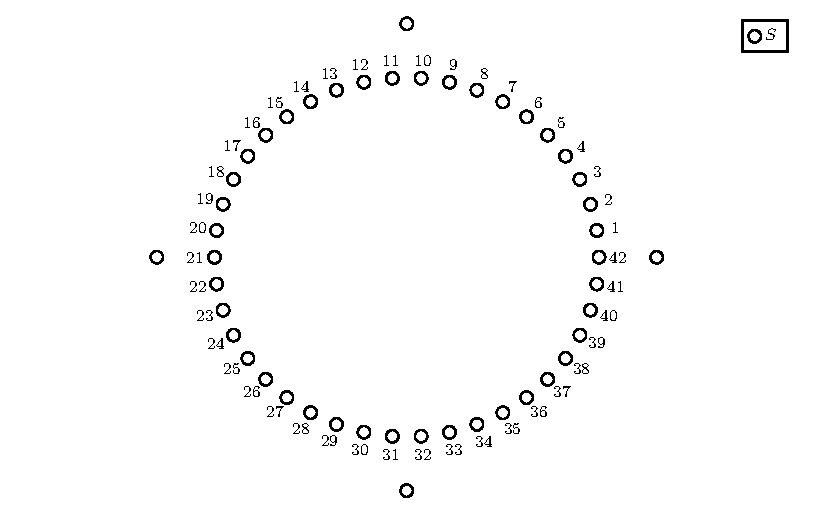
\includegraphics[scale = 0.6]{figures/circle_bijection.pdf}
    \caption{The points $(\cos(\theta_s), \sin(\theta_s))$ for $s \in S = \{1,\dots, 42\}$, where $\theta_s$ is defined by \eqref{eq:angle}.}\label{fig:circle-bijection}
\end{figure} 
Next, we endow $S$ with a metric $d:S \times S \to S$ defined by 
\begin{align*}
    d(s,t) = \min\left(t - s, s + n - t\right),\quad \quad s \leq t,
\end{align*}
or equivalently
\begin{align*}
    d(s,t) = \min\left(\max(s,t) - \min(s,t), \min(s,t) + n - \max(s,t)\right).
\end{align*}
Within the circle embedding, we may think of the the points as a graph with vertices $(\cos(\theta_s), \sin(\theta_s))$ for $s \in S$ and edges between each $(\cos(\theta_s), \sin(\theta_s))$ and $(\cos(\theta_{s + 1}), \sin(\theta_{s + 1}))$ for each $s \in \{1,\dots, n - 1\}$, aswell as an edge between $(\cos(\theta_n), \sin(\theta_n))$ and $(\cos(\theta_1), \sin(\theta_1))$; see Figure \ref{fig:circle-graph}.
\begin{figure}[ht]
    \centering
    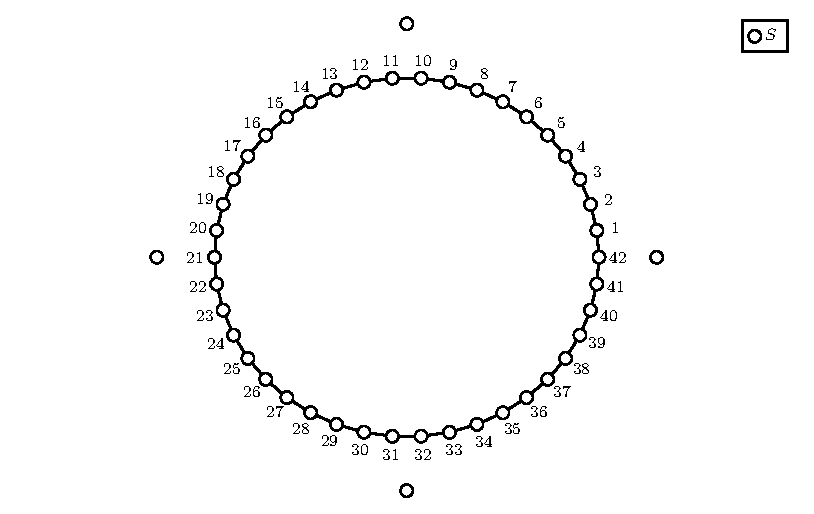
\includegraphics[scale = 0.6]{figures/circle_graph.pdf}
    \caption{The graph induced by adding edges between $(\cos(\theta_s), \sin(\theta_s))$ and $(\cos(\theta_{s + 1}), \sin(\theta_{s + 1}))$ for each $s \in \{1,\dots, n - 1\}$, aswell as an edge between $(\cos(\theta_n), \sin(\theta_n))$ and $(\cos(\theta_1), \sin(\theta_1))$.}\label{fig:circle-graph}
\end{figure}
Then, $d(s,t)$ corresponds to the number of edges one must traverse to travel from $s$ to $t$ in the undirected graph. Now, recall that $s \in A_{\oplus 1}$ if there exists an $a \in A$ such that $d(a,t) \leq R$. Hence, $A_{\oplus R}$ corresponds to the set of vertices $A$ as well as as the vertices which can be reached from a vertex in $A$ by traversing at most $R$ edges; we visualize in Figure \ref{fig:oplus_visualization}.\\\\ 
\begin{figure}[ht]
    \centering
    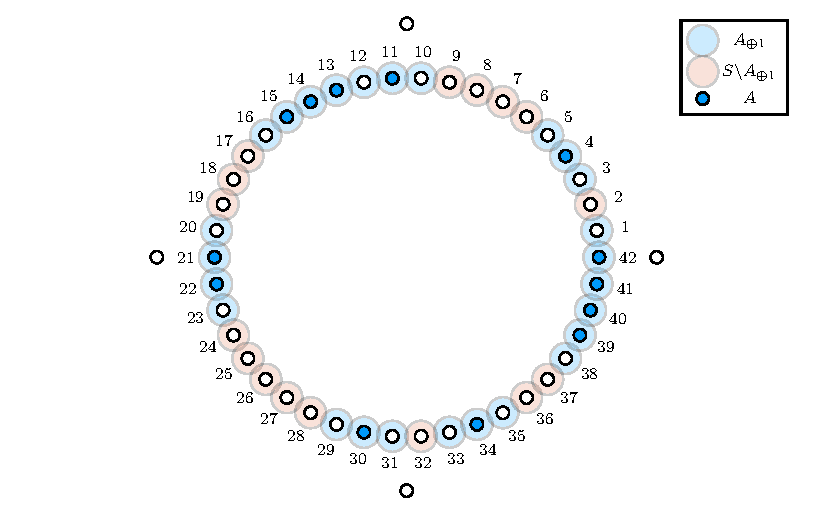
\includegraphics[scale = 0.6]{figures/oplus_visualization.pdf}
    \caption{The set $A_{\oplus 1}$ for a given set $A$ visualized in the circle.}\label{fig:oplus_visualization}
\end{figure}
Now, suppose that we are interested in simulating a point process on $S$ with the probability mass function  
\begin{align}\label{eq:pmf-area-interaction}
    p(A) = \frac{1}{Z} \beta^{|A|} \gamma^{-|A_{\oplus R}|}, \quad A \subseteq R,
\end{align}
where $\beta, \gamma,$ and $R$ are positive constants and $Z$ is a normalizing constant. Now, simulating from \eqref{eq:pmf-area-interaction} is hard for two reasons. First, if $n$ is large, it is not feasible to store all outcomes in memory, and in particular computing $Z$ is numerically intractable, c.f. the earlier remarks. Secondly, as the name suggests, there is an \textit{area interaction} enforced by the relationship between $\beta$ and $\gamma$. Of course, the trivial case $\gamma = 1$ is simple, as \eqref{eq:pmf-area-interaction} becomes $\frac{1}{Z}\beta^{|A|}$ which is a Poisson process with parameter $\beta$, for which each $X_s$ follows an i.i.d.  Bernoulli distribution with parameter $\frac{\beta}{1 + \beta}$ for all $s \in S$, which we can easily simulate by sampling each $X_s$ independently\footnote{This comment answers part 1 of Q5 and part 3 of Q1}. \newline\newline
To solve these problems, we introduce an auxiliary variable. 
\subsection*{Widom-Rowlinson Model}
For $X$ following an area-interaction process, we will now consider an auxiliary variable approach leading to the so-called Widom-Rowlinson model. \newline\newline
Within the Widom-Rowlinsom model, we also consider a finite metric space $(S,d)$. Let $Y_1$ and $Y_2$ denote two independent Poisson processes on $S$ and condition on $d(Y_1, Y_2) = \min_{s \in Y_1, t \in Y_2} d(s,t) > R$ for some $R > 0$ called the hard-core; intuitively, the condition separates the two otherwise independent Poisson process, forcing them to keep at least a distance of $R$ to one-another. \\\\
Now, let us derive the probability mass function for the conditioned process. Note, that 
\begin{align*}
    \mathbb{P}(Y_1 = A_1, Y_2 = A_2 \mid d(Y_1, Y_2) > R) &= \frac{\mathbb{P}(Y_1 = A_1, Y_2 = A_2, d(Y_1, Y_2) > R)}{\mathbb{P}(d(Y_1, Y_2) > R)}\\
    &\propto \mathbb{P}(Y_1 = A_1, Y_2 = A_2, d(Y_1, Y_2) > R) \\
    &= \mathbb{P}(Y_1 = A_1, Y_2 = A_2, d(A_1, A_2) > R)\\
    &=\mathbb{P}(Y_1 = A_1, Y_2 = A_2)\mathbbm{1}[d(A_1, A_2) > R]\\
    &= \mathbb{P}(Y_1 = A_1) \mathbb{P}(Y_2 = A_2) \mathbbm{1}[d(A_1, A_2) > R],
\end{align*} 
where the first equation follows by definition. The proportionaly then simply ignores the fixed divisor. Subsequently, the joint distribution of $\mathbb{P}(Y_1 = A_1, Y_2 = A_2, d(Y_1, Y_2) > R)$ can be written as $\mathbb{P}(Y_1 = A_1, Y_2 = A_2, d(A_1, A_2) > R)$, as we consider a joint distribution. However, the term $d(A_1, A_2) > R$ is no longer random, in the sense that it is either true or false for a given $A_1$ and $A_2$. Hence, we can rewrite $\mathbb{P}(Y_1 = A_1, Y_2 = A_2, d(A_1, A_2) > R) = \mathbb{P}(Y_1 = A_1, Y_2 = A_2)\mathbbm{1}[d(A_1, A_2) > R]$. The final equality then follows from the independence of $Y_1$ and $Y_2$ prior to the hard-core condition\footnote{This answers the $1^{\mathrm{st}}$ question in Q2}. Notice, that if we condition on $Y_2 = A$, we have  
\begin{align*}
    \mathbb{P}(Y_1 = A_1 \mid Y_2 = A, d(Y_1, Y_2) > R) \propto \beta_1^{|A_1|} \mathbbm{1}[d(A_1, A) > R],
\end{align*}
for all $A_1 \subseteq S$. However, if $A_1 \subseteq  S \backslash A_{\oplus R}$, then clearly $d(A_1, A) > R$; it corresponds to the set-difference between $S$ and $A_{\oplus R}$, where the latter is defined by all the points $s$ for which there exists an $a \in A$ such that $d(s,a) \leq R$. Hence, for $s$ in the complement $S\backslash A_{\oplus R}$ we must have $d(s,a) > R$ for all $a \in A$. Therefore, we have for $A_1 \subseteq S \backslash A_{\oplus R}$ we have 
\begin{align*}
    \mathbb{P}(Y_1 = A_1 \mid Y_2 = A, d(Y_1, Y_2) > R) \propto \beta_1^{|A_1|},
\end{align*}
which coincides with the probability mass function of a Poisson process on $S$ with parameter $\beta_1$. Hence, conditioned on $Y_2 = A$, we have that $Y_1$ is a Poisson process with parameter $\beta_1$ on $S\backslash A_{\oplus R}$. Analogous arguments show that conditioned on $Y_1 = A$, we have that $Y_2$ is a Poisson process on $S\backslash A_{\oplus R}$ with parameter $\beta_2$.\footnote{This answers the $2^{\mathrm{nd}}$ point of Q2.}. \newline\newline 
In particular, since $Y_1$ and $Y_2$ were independent, but we later condition on the hard-core condition, we can first simulate $Y_1$, which was assumed to be a Poisson process on $S$ with parameter $\beta_1$, which yields and outcome $Y_1 = A$. Then, we can subsequently simulate $Y_2$ on $S\backslash A_{\oplus R}$ as a Poisson process with parameter $\beta_2$. Then, the pair $(Y_1, Y_2)$ will follow the joint distribution obeying the hard-core condition.\footnote{This answers the $3^{\mathrm{rd}}$ question in Q2.}\newline\newline
Now, let us derive the conditional probability mass function of $Y_1$ given the hard-core condition. To this end, notice that 
\begin{align*}
    \mathbb{P}(Y_1 = A \mid d(Y_1, Y_2) > R) &=  \sum_{B \in \wp(S)} \mathbb{P}(Y_1 = A, Y_2 = B \mid d(Y_1, Y_2) > R)\\
    &\propto \sum_{B \in \wp(S)} \beta_1^{|A|}\beta_2^{|B|}\mathbbm{1}[d(A,B) > R]\\
    &=\beta_1^{|A|} \sum_{B \in \wp(S)} \beta_2^{|B|} \cdot \mathbbm{1}[d(A,B) > R]\\
    &=\beta_1^{|A|} \sum_{B \subseteq S\backslash A_{\oplus R}} \beta_2^{|B|}\\
    &= \beta_1^{|A|} \cdot \sum_{n = 0}^{|S \backslash A_{\oplus R}|} \begin{pmatrix}
        |S \backslash A_{\oplus R}|\\
        n
    \end{pmatrix}\beta^n\\
    &= \beta_1^{|A|} (1+\beta_2)^{|S \backslash A_{\oplus R}|}\\
    &\propto\beta_1^{|A|} (1+\beta_2)^{-|A_{\oplus R}|},
\end{align*}
which gives us a marginal distribution for $Y_1$, albeit still conditional on the hard-core condition. One shows that
\begin{align*}
    \mathbb{P}(Y_2 = A \mid d(Y_1,Y_2)>R) \propto\beta_2^{|A|} (1+\beta_1)^{-|A_{\oplus R}|}
\end{align*}
analogously.\footnote{This answers all the questions in Q4.}
Now, notice that the last proportionality coincides exactly with the area-interaction model when $\gamma > 1$; set $\gamma = (1 + \beta_2)$ and notice that the proportionality accounts for the normalizing constant.\footnote{This answers the $2^{\mathrm{nd}}$ question in Q5.}\newline\newline
In particular, we can, conditioned on the hard-core condition, consider $Y_2$ (or $Y_1$) as an auxiliary variable for the area-interaction process with $\gamma > 1$; set $X = Y_1$ and let $Y_2$ be the auxiliary variable, where we implicitly assume that $Y_1$ and $Y_2$ are conditioned on the hard-core condition. \footnote{This answers Q16.}
\subsection{Simulation from the Widom-Rowlinson}
Now, we consider a Gibbs sampler for the Widom-Rowlinsom model. We exemplify using the space $S = \{1,\dots, n\}$ which we embed on the circle using the transformation 
\begin{align*}
    s \mapsto (\cos(\theta_s), \sin(\theta_s)), \quad \theta_s = \frac{2\pi s}{n}.
\end{align*}
The simulation is then carried out as follows: 
\begin{itemize}
    \item[(i)] Initialize $Y_1$; we choose to sample $Y_1$ as a Poisson process on $S$ with parameter $\beta_1$.
    \item[(ii)] Sample $Y_2$ as a Poisson process with parameter $\beta_2$ on $S\backslash (Y_{1})_{\oplus R}$. 
    \item[(iii)] Sample $Y_1$ as a Poisson process with parameter $\beta_1$ on $S\backslash (Y_{2})_{\oplus R}$.
    \item[(iv)] Alternate points (ii) and (iii).  
\end{itemize}
We implement below in the \texttt{Julia} programming language.
%\bibliographystyle{abbrv}
%bibliography{incl/bib/articles}

\end{document}